\begin{frame}{Modelling}{Introduction}
	\begin{itemize}
		\item First principles modelling
		\item Only dynamics relevant to fore-aft motion included
		\item Component modelled and linearised individually
		\item Only fore-aft motion model included in presentation
	\end{itemize}
\end{frame}

%%%%%%%%%%%%%%%%

\begin{frame}{Modelling}{Tower fore-aft motion}
	\begin{equation}
		\begin{split}
			\dot{v}_y & = \dfrac{F_{rot} - b v_y - k p_y}{m} \\
			\dot{p}_y & = v_y
		\end{split}
	\end{equation}
	\begin{equation}
			k = (2 \pi f_{eig})^2 m \;\; , \;\; b = 2 \zeta \sqrt{k m}
	\end{equation}
	\begin{figure}[ht]
		\centering
		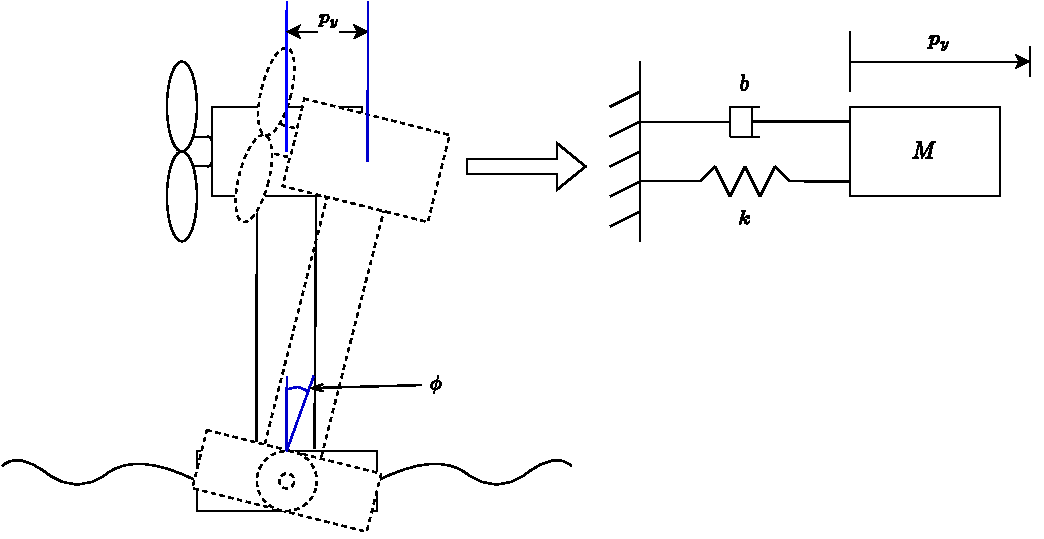
\includegraphics[width=0.9\linewidth]{../Graphics/wtLinForeAftMotionModel.pdf}
		\label{fig:wtLin_fore-aft_diagram}
	\end{figure}
\end{frame}

%%%%%%%%%%%%%%%%

\begin{frame}{Modelling}{Fore-aft model fitting}
	Fore-aft motion model parameter fitting results:
	\begin{columns}
		\begin{column}{.49\textwidth}
			\begin{figure}[ht]
				\centering
				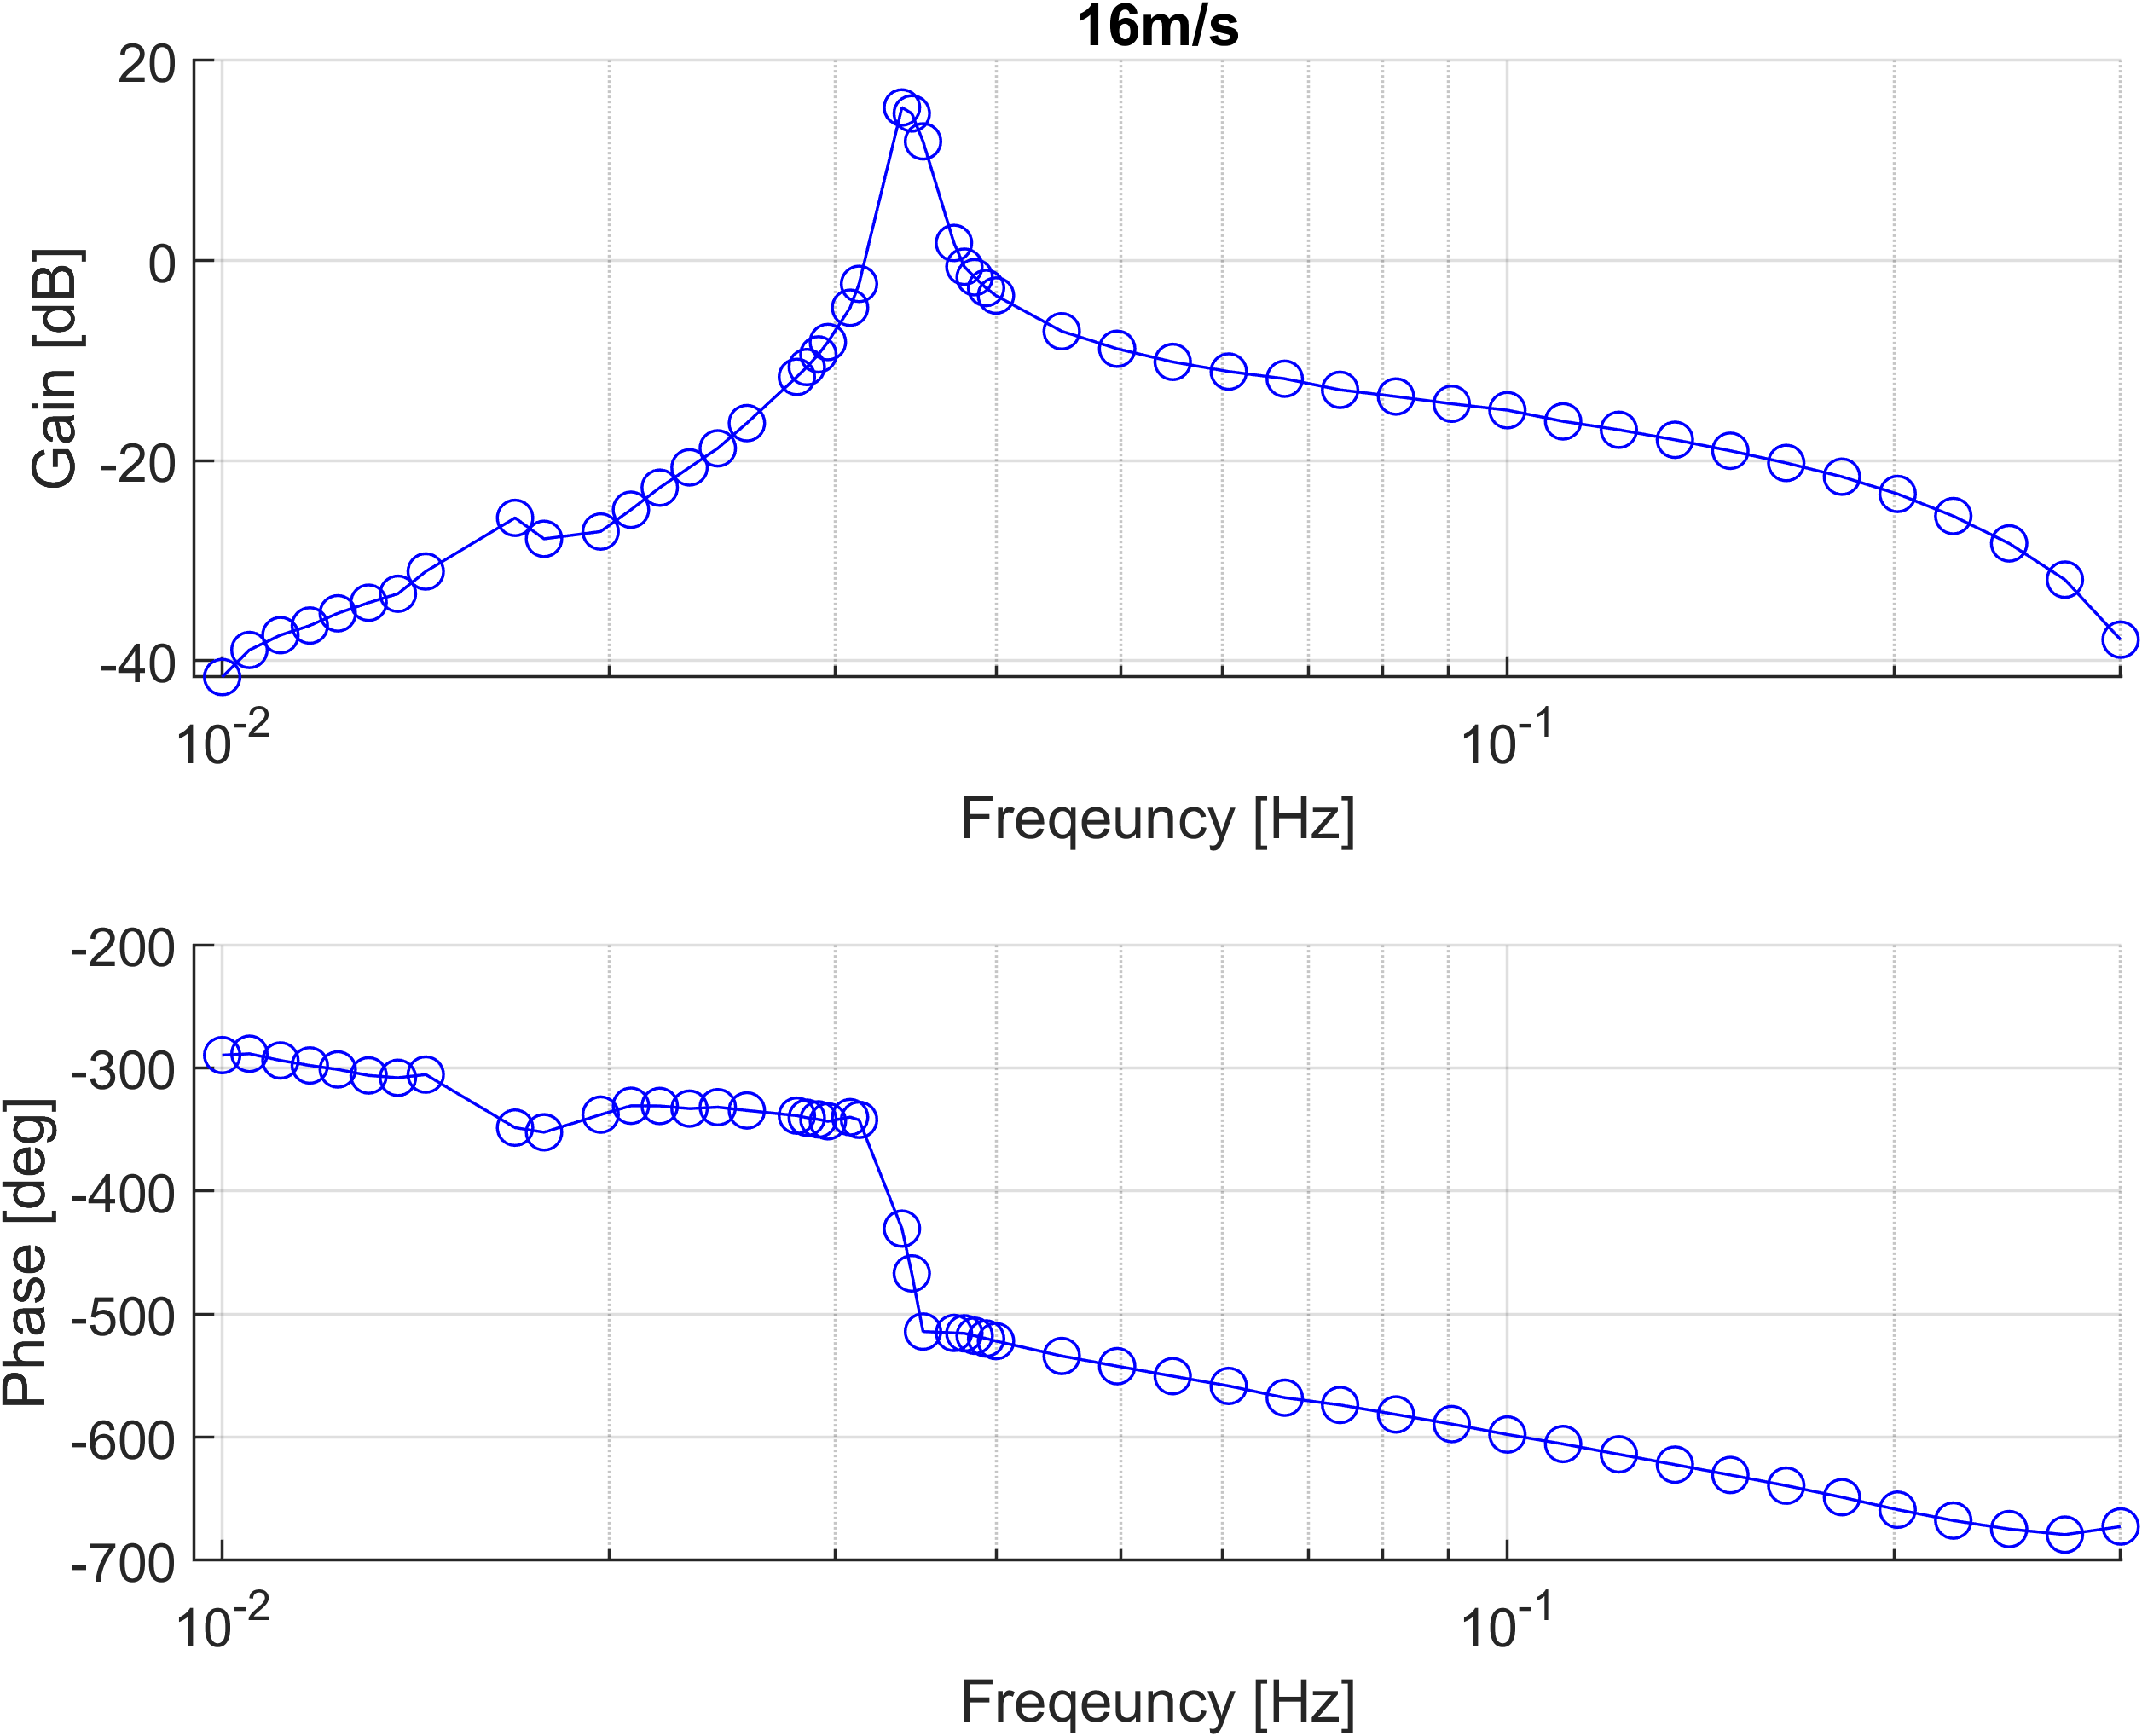
\includegraphics[width=1\linewidth]{../Graphics/TestResults/foreaftFitting/sysid_thSine-vy_16ms.png}
				\label{fig:sysid_wref-vy_16}
			\end{figure}
			\centering VTS
		\end{column}
	
		\begin{column}{.49\textwidth}
			\begin{figure}[ht]
				\centering
				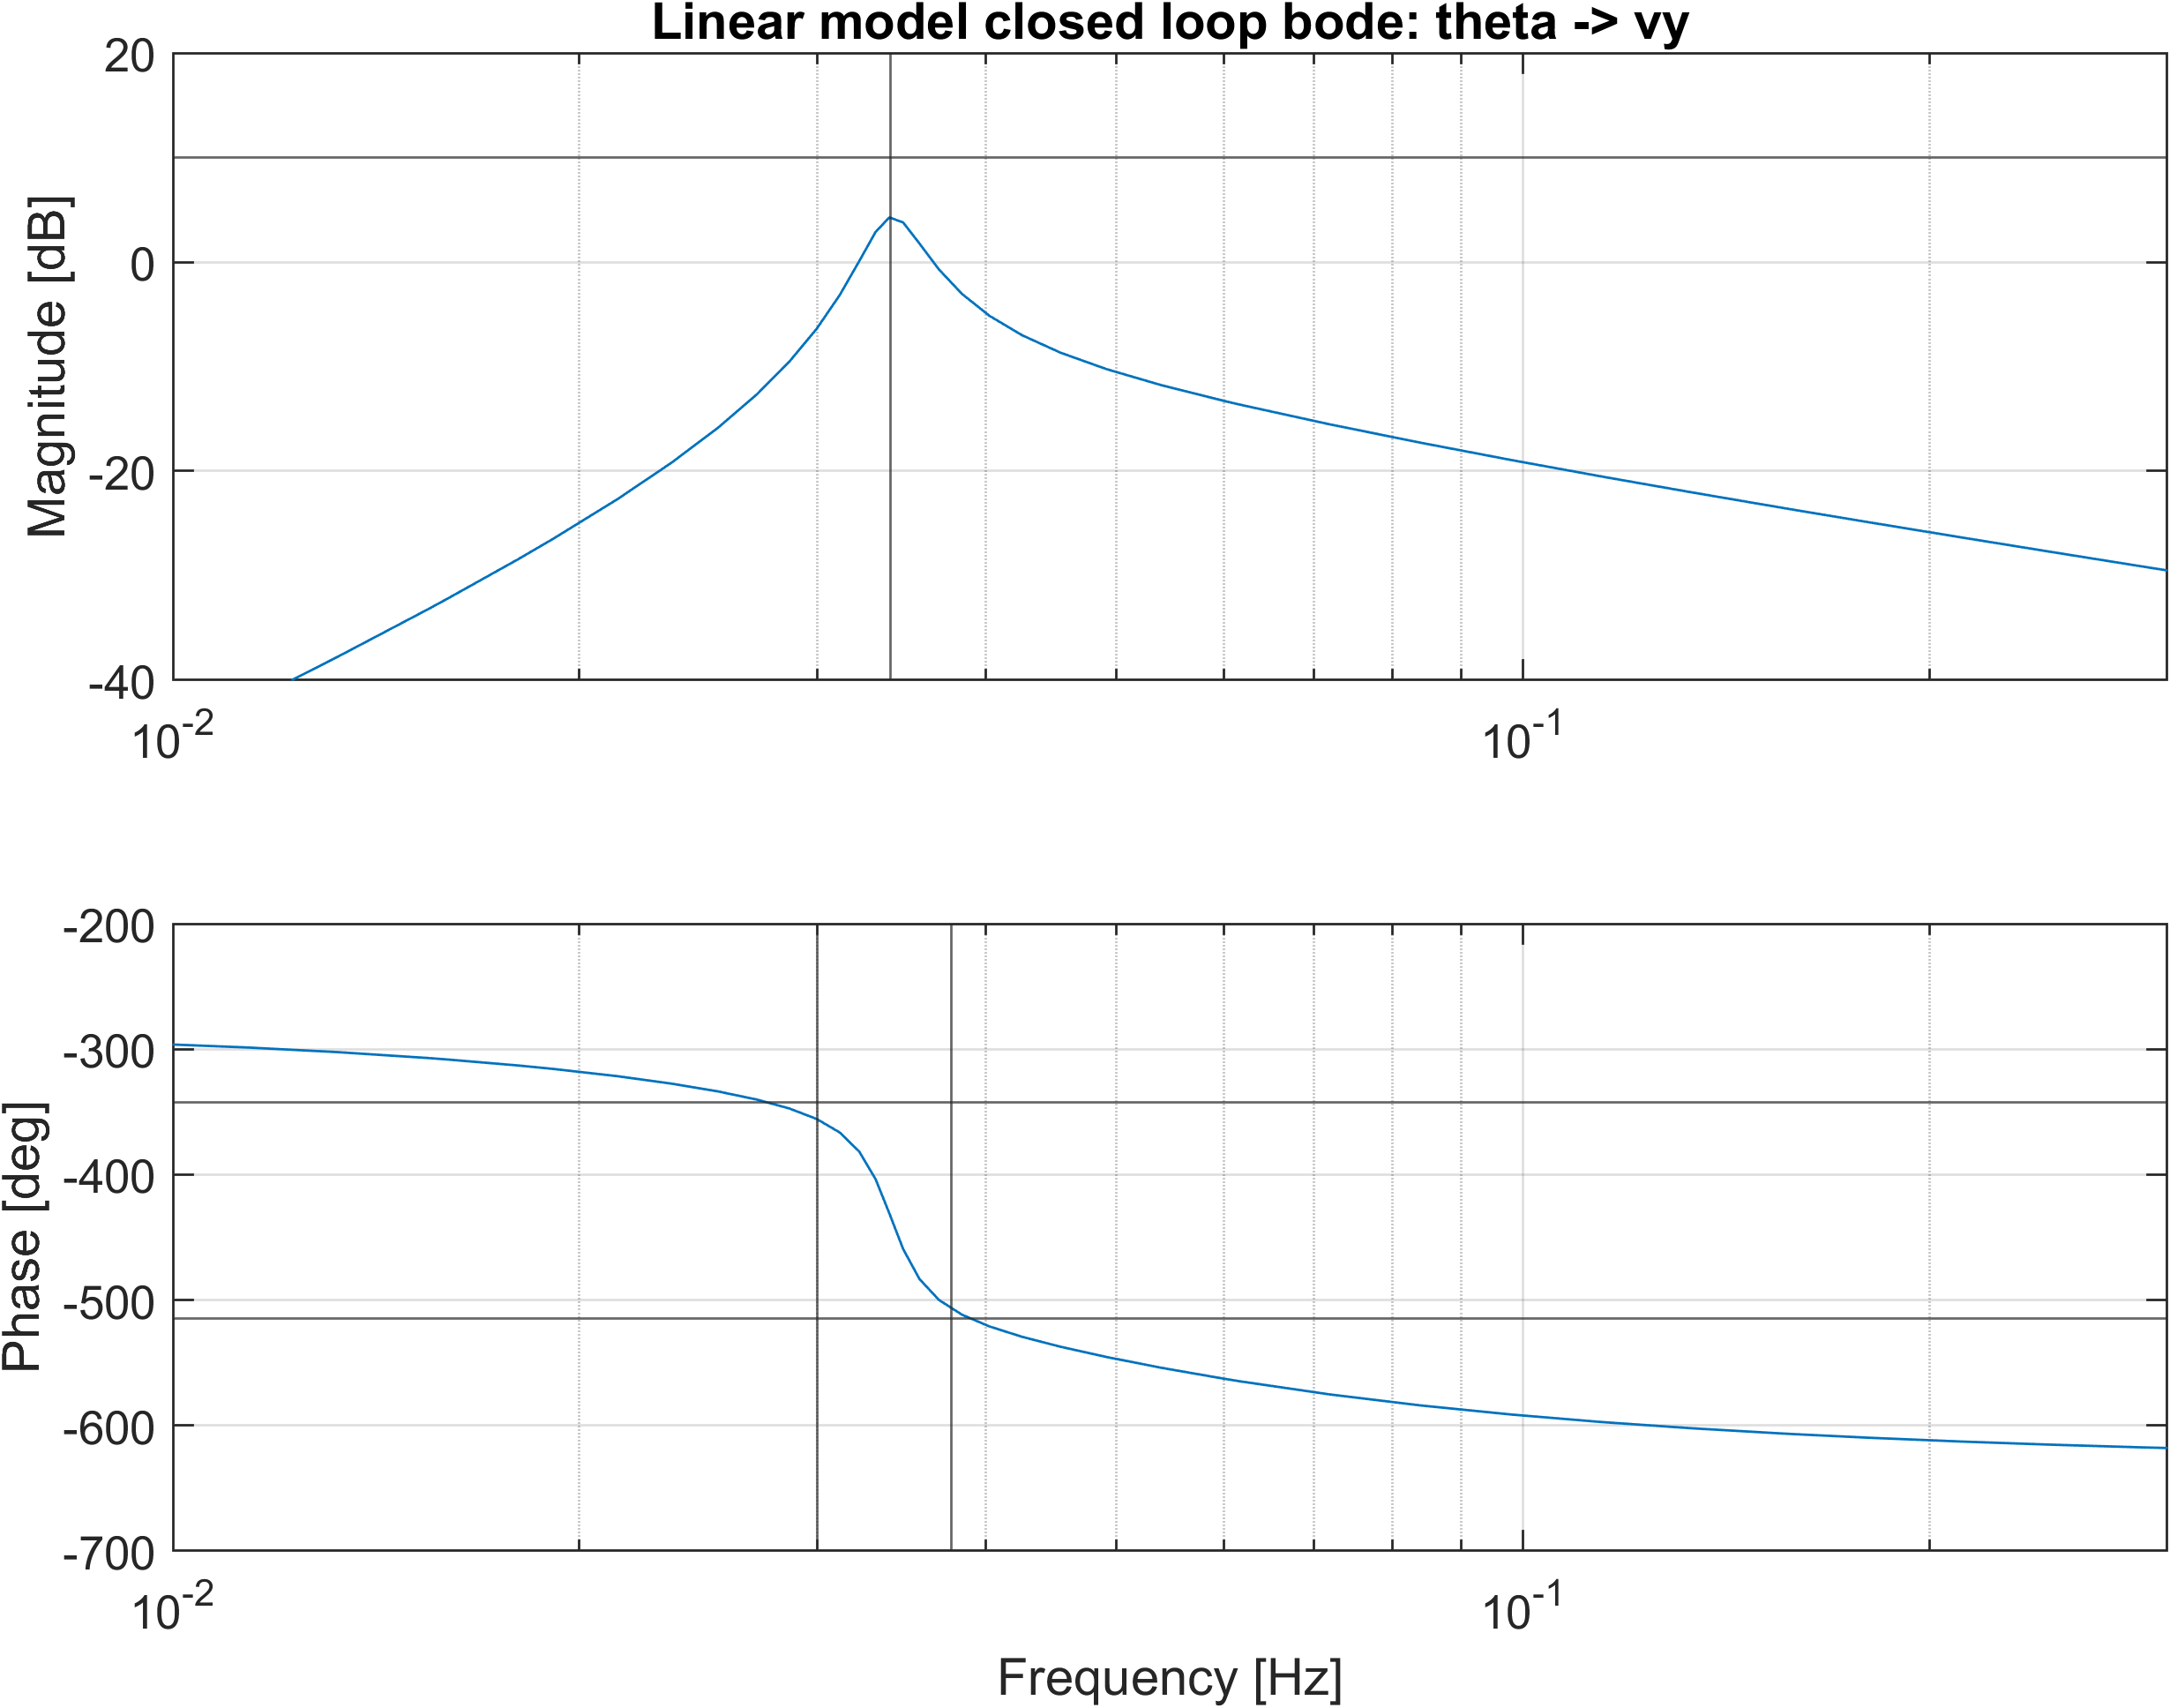
\includegraphics[width=1\linewidth]{../Graphics/TestResults/foreaftFitting/wtLin_th-vy_16ms.png}
				\label{fig:wtlin_wref-vy_16}
			\end{figure}
			\centering Linear model
		\end{column}
	\end{columns}
	
\end{frame}

%%%%%%%%%%%%%%%%

\begin{frame}{Modelling}{The model}
	The resulting state-space model:
	\begin{itemize}
		\item \textbf{States:} \{$ p_y, v_y, \Omega, \Omega_{int} $\} \hspace{1mm} with $ \Omega =$ rotor speed
		\item \textbf{Input:} \{$ \omega_{ref} $\} \hspace{1mm} with $ \omega =$ generator speed
		\item \textbf{Disturbance:} \{$ v_{free} $\}
		\item \textbf{Outputs:} \{$ p_y, v_y, \Omega $\}
		\item Stable
		\item Controllable and observable
	\end{itemize}	
\end{frame}